\documentclass{book}

\usepackage{amssymb}
\usepackage{amsmath}
\usepackage{amsthm}
\usepackage{arydshln}
\usepackage{calc}
\usepackage{cancel}
\usepackage{caption}
\usepackage{cite}
\usepackage{color}
\usepackage{enumitem}
\usepackage{esint}
\usepackage{etoolbox}
\usepackage{float}
\usepackage{framed}
\usepackage{fullpage}
\usepackage{gensymb}
\usepackage[margin=1in]{geometry}
\usepackage{graphicx}
\usepackage{listings}
\usepackage{multirow}
\usepackage{subfiles}
\usepackage{rsfso}
\usepackage{tikz}
\usepackage{tikz-3dplot}
\usepackage{ushort}
\usepackage{wrapfig}
\usepackage{xcolor}
\usepackage{soul}
\usepackage{epstopdf}

% pdf versions
\pdfoptionpdfminorversion=7

% handle page stretching
\raggedbottom

% Graphics file location
\graphicspath{{Graphics/}{../Graphics/}}

% Use for drawings
\usetikzlibrary{angles,arrows,calc,decorations,intersections,patterns,positioning,quotes,shapes}
\usetikzlibrary{shapes.geometric}
\usetikzlibrary{decorations.pathreplacing}
\newcommand{\midarrow}{\tikz \draw[-latex] (0,0) -- +(.1,0);}

% Tikz commands for drawing block diagrams, etc...
\tikzset{%
	block/.style    = {draw, rectangle, minimum height = 2em, minimum width = 2em},
	sum/.style      = {draw, circle}, % Adder
	input/.style    = {fill=white, rectangle}, % Input
	output/.style   = {fill=white, rectangle}, % Output
	waypoint/.style   = {coordinate}, % Output
}

\tikzset{%
	startstop/.style= {draw, rectangle, rounded corners, minimum width=2cm, minimum height=1cm,text centered},
	inout/.style    = {draw, trapezium, trapezium left angle=70, trapezium right angle=110, minimum width=2cm, minimum height=1cm, text centered},
	process/.style  = {draw, rectangle, minimum width=2cm, minimum height=1cm, text centered},
	decision/.style = {draw, diamond, minimum width=1.5cm, minimum height=1cm, text centered, diamond, aspect=2},
	arrow/.style    = {thick,-latex,>=stealth},		
}

\tikzset{
	saveuse path/.code 2 args={
		\pgfkeysalso{#1/.style={insert path={#2}}}%
		\global\expandafter\let\csname pgfk@\pgfkeyscurrentpath/.@cmd\expandafter\endcsname
		% not optimal as it is now global through out the document
		\csname pgfk@\pgfkeyscurrentpath/.@cmd\endcsname
		\pgfkeysalso{#1}},
	/pgf/math set seed/.code=\pgfmathsetseed{#1}}

% Define Laplace, Fourier transform symbols
\newcommand{\LT}{\mathcal{L}}
\newcommand{\FT}{\mathcal{F}}

% Define adjugate function
\newcommand{\adj}{\text{adj}}

% Define rank function
\newcommand{\rank}{\text{rank}}

% commands to speed up writing j\omega and s-plane
\newcommand{\jw}{j\omega}
\newcommand{\jt}{j\theta}
\newcommand{\wt}{\omega t}
\newcommand{\spl}{s\textrm{-plane}}
\newcommand{\Lm}{\textrm{Lm }}
% Clean up overline/underline for math mode
\def\obar#1{\bar{#1}}
\def\ubar#1{\ushort{#1}}

\newcommand{\exmp}{\subsubsection*{Example}}
\newcommand{\nib}{\noindent$ \bullet\ $}


\begin{document}
\chapter*{Lecture 2}
Last time:
\begin{itemize}
	\item Painted a picture of what this course is about, and where we are going with it.
	\item Started with a review of the Laplace Transform
	\[ L[f(t)] = \int_{0^-}^{\infty} e^{-st}f(t)dt \]
	\item Did an example to show that $ L[1(t)]=1/s $
	\item Also listed a few useful LT theorems:
	\begin{itemize}
		\item $ \LT[e^{-at}f(t)]=F(s+a) $ where $ a $ is constant
		\item $ \LT[tf(t)]=-\frac{d}{ds}F(s) $
		\item $ \LT[t^nf(t)]=(-1)^n\frac{d^n}{ds^n}F(s) $
		\item $ \LT[af(t)+bg(t)]=aF(s)+bG(s) $ where $ a $ and $ b $ are constant
		\item $ \LT[\frac{d}{dt}f(t)]=sF(s)-f(0^-) $
		\item $ \LT[\frac{d^2}{dt^2}f(t)]=s^2F(s)-sf(0^-)-\frac{df}{dt}(0^-) $
		\item $ \LT[\frac{d^n}{dt^n}f(t)]=s^nF(s)-\sum_{k=1}^n s^{n-k}\frac{d^{k-1}f}{dt^{k-1}}(0^-) $
		\item $ \LT[\int_{0^-}^t f(\tau) d\tau]=\frac{F(s)}{s} $
	\end{itemize}
	\item We can express $ s $-domain functions using a \textbf{pole-zero diagram}.
	\begin{center}
		\begin{tikzpicture}[scale=1]
		\draw (-5,0) -- (2,0) node[below left] {$ \sigma $};
		\draw (0,-1.5) -- (0,1.5) node[below left] {$ j\omega $};
		\node at (-4,0) {\Large$ \times $};
		\node at (-1,0) {\Large$ \times $};
		\node at (-2,0) {\Large$ \circ $};
		
		\node[align=left] at (-4,1.25) {\Large$ \circ $:\normalsize Zeros};
		\node[align=left] at (-4,0.875) {\Large$ \times $:\normalsize Poles};
		\end{tikzpicture}
	\end{center}
\end{itemize}

How would we transform the sine and cosine functions?
\[ f(t) = \sin\wt\ 1(t) \Rightarrow F(s) =  \]
\[ g(t) = \cos\wt\ 1(t) \Rightarrow G(s) =  \]
Let's use Euler's Identity, also called Euler's Theorem:
\[ e^{j\theta} = \cos\theta + j\sin\theta \]
\[ e^{-j\theta} = \cos\theta - j\sin\theta \]
Add/subtract:
\[ \cos\theta = \frac{e^{j\theta}+e^{-j\theta}}{2} \]
\[ \sin\theta = \frac{e^{j\theta}-e^{-j\theta}}{2j} \]
So,
\begin{align*}
\LT[\cos\wt\ 1(t)] &= \LT[\frac{1}{2}(e^{j\wt}+e^{-j\wt})1(t)]\\
&= \frac{1}{2}\LT[e^{\jw t}1(t)]+\frac{1}{2}\LT[e^{-\jw t}1(t)]\\
&=\frac{1/2}{s-\jw}+\frac{1/2}{s+\jw}\\
&=\frac{s}{s^2+\omega^2}
\end{align*}
Hence,
\[ \LT[\cos\wt\ 1(t)] = \frac{s}{s^2+\omega^2} \]
\begin{center}
	\begin{tikzpicture}[scale=2]
	\draw[->] (-0.5,0) -- (2,0);  % x Axis
	\draw[->] (0,-0.625) -- (0,0.625);  % y Axis
	\node[below left ] at (2,0) {$ t $};
	\node[below left] at (0,0.625) {$ f(t) $};
%	\node[above] at (1,0.5) {$ e^{-at} $};
	
	\draw[domain=0:2,samples=240] plot (\x,{.375*cos((180/pi)*8*\x)});
	
	\begin{scope}[shift={(4.5cm,0.0cm)},scale=0.5]
	\draw[<->] (-2.5,0) -- (2.5,0) node[below left] {$ \sigma $};
	\draw[<->] (0,-1.5) -- (0,1.5) node[below left] {$ j\omega $};
	\node at (0,1) {\Large$ \times $};
	\node at (0,-1) {\Large$ \times $};
	\node at (0,0) {\Large$ \circ $};
	\end{scope}
	
	\end{tikzpicture}
\end{center}

Similarly we can show that
\begin{align*}
\LT[\sin\wt\ 1(t)] &= \LT[\frac{1}{2j}(e^{j\theta}-e^{-j\theta})1(t)]\\
&= \frac{1}{2j}\LT[e^{\jw t}1(t)]-\frac{1}{2j}\LT[e^{-\jw t}1(t)]\\
&=\frac{1}{2j}\frac{1}{s-\jw}+\frac{1}{2j}\frac{1}{s+\jw} = \frac{1}{2j}\frac{s+\jw-s+\jw}{(s-\jw)(s+\jw)}\\
&=\frac{\omega}{s^2+\omega^2}
\end{align*}
\begin{center}
	\begin{tikzpicture}[scale=2]
	\draw[->] (-0.5,0) -- (2,0);  % x Axis
	\draw[->] (0,-0.625) -- (0,0.625);  % y Axis
	\node[below left] at (2,0) {$ t $};
	\node[below left] at (0,0.625) {$ f(t) $};
	%	\node[above] at (1,0.5) {$ e^{-at} $};
	
	\draw[domain=0:2,samples=240] plot (\x,{.375*sin((180/pi)*8*\x)});
	
	\begin{scope}[shift={(4.5cm,0cm)},scale=0.5]
	\draw[<->] (-2.5,0) -- (2.5,0) node[below left] {$ \sigma $};
	\draw[<->] (0,-1.5) -- (0,1.5) node[below left] {$ j\omega $};
	\node at (0,1) {\Large$ \times $};
	\node at (0,-1) {\Large$ \times $};
%	\node at (0,0) {\Large$ \circ $};
	\end{scope}
	
	\end{tikzpicture}
\end{center}

We are now in a position to determine the Laplace Transform of most of the functions that are encountered in the study of LTI systems.

\subsection*{Proof of the Euler Identity}
The subsection covers the proof of the Euler Identity, used in the previous example. Start with the Taylor series expansion of $ e^x $.
\[ e^x = 1+x+\frac{x^2}{2!}+\frac{x^3}{3!}+\ldots+\frac{x^n}{n!}+\ldots \]
So,
\begin{align*}
e^{\jt} & = 1+\jt+\frac{(\jt)^2}{2!}+\frac{(\jt)^3}{3!}+\ldots\\
&= 1+\jt - \frac{\theta^2}{2!}-\frac{\jt^3}{3!}+\frac{\theta^4}{4!}+\ldots\\
&=\underbrace{1- \frac{\theta^2}{2!}+\frac{\theta^4}{4!} - \frac{\theta^6}{6!}+\ldots}_{\cos\theta} + j \underbrace{\jt-\frac{\jt^3}{3!}+\frac{\jt^5}{5!} - \ldots}_{\sin\theta}\\
e^{\jt} & = \cos\theta+j\sin\theta\\
e^{-\jt} & = \cos\theta-j\sin\theta
\end{align*}
So,
\[ \cos\theta = \frac{e^{j\theta}+e^{-j\theta}}{2},\quad \sin\theta = \frac{e^{j\theta}-e^{-j\theta}}{2} \]

\subsection*{Summary So Far}
Let's summarize our results so far into a table.
\begin{center}
	\begin{tabular}{c c c c}
	Function $ f(t) $ & Plot of $ f(t) $ & $ F(s) $ & Pole-Zero Diagram \\ \hline\vspace{0.5em}
	$ \delta(t) $ & 	\begin{tikzpicture}[scale=1]
	\draw[->] (-0.5,0) -- (2,0);  % x Axis
	\draw[->] (0,-0.25) -- (0,1.0);  % y Axis
	\node[below] at (1.9,0) {$ t $};
	\node[left] at (0,0.9) {$ f(t) $};
	\draw[ultra thick,->] (0,0) -- (0,0.75);
	\end{tikzpicture}
	& $ 1 $ & (no poles or zeros) \\ \hline\vspace{0.5em}
	$ 1(t) $ & 	\begin{tikzpicture}[scale=1]
	\draw[->] (-0.5,0) -- (2,0);  % x Axis
	\draw[->] (0,-0.25) -- (0,1.0);  % y Axis
	\node[below] at (1.9,0) {$ t $};
	\node[left] at (0,0.9) {$ f(t) $};
	\draw[domain=0:2] plot (\x,{.75});
	\end{tikzpicture}
	 & $ \dfrac{1}{s} $ & \begin{tikzpicture}[scale=0.5]
	 \draw (-2.5,0) -- (2.5,0) node[below left] {$ \sigma $};
	 \draw (0,-1.5) -- (0,1.5) node[below left] {$ j\omega $};
	 \node at (0,0) {\Large$ \times $};
	 \end{tikzpicture} \\ \hline\vspace{0.5em}
	$ e^{-at}1(t) $ & 	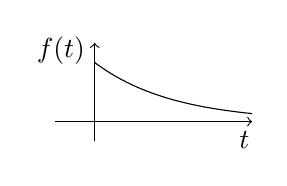
\begin{tikzpicture}
	\draw[->] (-0.5,0) -- (2,0);  % x Axis
	\draw[->] (0,-0.25) -- (0,1.0);  % y Axis
	\node[below] at (1.9,0) {$ t $};
	\node[left] at (0,0.9) {$ f(t) $};
	\draw[domain=0:2] plot (\x,{.75*exp(-\x)});
	\end{tikzpicture} & $ \dfrac{1}{s+a} $ & 	\begin{tikzpicture}[scale=0.5]
	\draw (-3,0) -- (2,0) node[below left] {$ \sigma $};
	\draw (0,-1.5) -- (0,1.5) node[below left] {$ j\omega $};
	\node at (-1,0) {\Large$ \times $};
	\node[below] at (-1,0) {$ a $};
	\end{tikzpicture} \\ \hline\vspace{0.5em}
	$ t1(t) $ & 	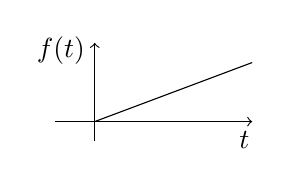
\begin{tikzpicture}
	\draw[->] (-0.5,0) -- (2,0);  % x Axis
	\draw[->] (0,-0.25) -- (0,1.0);  % y Axis
	\node[below] at (1.9,0) {$ t $};
	\node[left] at (0,0.9) {$ f(t) $};
	\draw[domain=0:2] plot (\x,{.375*\x});
	\end{tikzpicture} & $ \dfrac{1}{s^2} $ & 	\begin{tikzpicture}[scale=0.5]
	\draw (-3,0) -- (2,0) node[below left] {$ \sigma $};
	\draw (0,-1.5) -- (0,1.5) node[below left] {$ j\omega $};
	\node at (0,0) {\Large$ \times $};
	\node[above right] at (0,0) {$ 2 $};
	\end{tikzpicture} \\ \hline\vspace{0.5em}
	$ \cos\wt1(t) $ & 	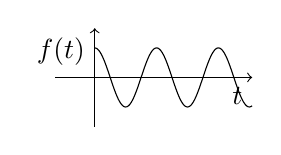
\begin{tikzpicture}[scale=1]
	\draw[->] (-0.5,0) -- (2,0);  % x Axis
	\draw[->] (0,-0.625) -- (0,0.625);  % y Axis
	\node[below left ] at (2,0) {$ t $};
	\node[below left] at (0,0.625) {$ f(t) $};
	\draw[domain=0:2,samples=240] plot (\x,{.375*cos((180/pi)*8*\x)});
	\end{tikzpicture} & $ \dfrac{s}{s^2+\omega^2} $ & 	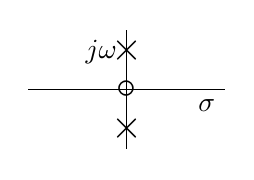
\begin{tikzpicture}[scale=0.5]
	\draw (-2.5,0) -- (2.5,0) node[below left] {$ \sigma $};
	\draw (0,-1.5) -- (0,1.5) node[below left] {$ j\omega $};
	\node at (0,1) {\Large$ \times $};
	\node at (0,-1) {\Large$ \times $};
	\node at (0,0) {\Large$ \circ $};
	\end{tikzpicture} \\ \hline\vspace{0.5em}
	$ \sin\wt1(t) $ & 	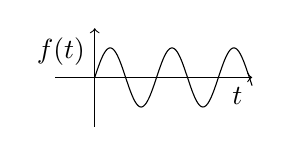
\begin{tikzpicture}
	\draw[->] (-0.5,0) -- (2,0);  % x Axis
	\draw[->] (0,-0.625) -- (0,0.625);  % y Axis
	\node[below left] at (2,0) {$ t $};
	\node[below left] at (0,0.625) {$ f(t) $};
	\draw[domain=0:2,samples=240] plot (\x,{.375*sin((180/pi)*8*\x)});
	\end{tikzpicture} & $ \dfrac{\omega}{s^2+\omega^2} $ & 	\begin{tikzpicture}[scale=0.5]
	\draw (-2.5,0) -- (2.5,0) node[below left] {$ \sigma $};
	\draw (0,-1.5) -- (0,1.5) node[below left] {$ j\omega $};
	\node at (0,1) {\Large$ \times $};
	\node at (0,-1) {\Large$ \times $};
	\end{tikzpicture} \\
	
	
	\end{tabular}
\end{center}

We will now do some examples of the Laplace Transform.

\exmp
\[ f(t) = t^2+e^{-2t}\sin3t \]
Find the Laplace transform of $ f(t) $. $ f(t) $ can be written formally (in causal form) as
\[ f(t) = t^21(t)+e^{-2t}\sin3t1(t) \qquad\qquad(1) \]
So,
\begin{align*}
\LT[1(t)]&=\frac{1}{s}&(2)\\
\LT[t\cdot 1(t)]&=-\frac{d}{ds}\frac{1}{s}=\frac{1}{s^2}&(3)\\
\LT[t\cdot t\cdot 1(t)]&=-\frac{d}{ds}\frac{1}{s^2}=\frac{2}{s^3}&(4)\\
\LT[\sin 3t\cdot 1(t)]&=\frac{3}{s^2+3^2}=\frac{3}{s^2+9}&(5)\\
\LT[e^{-2t}\cdot\sin 3t\cdot 1(t)]&=\frac{3}{(s+2)^2+3^2}=\frac{3}{(s+2)^2+9}&(6)\\
\end{align*}
From (1), (4), and (6):
\[ F(s) = \frac{2}{s^3} + \frac{3}{(s+2)^2+9} \]


\exmp
We want to solve: 
\[ \ddot{y}(t) + 5\dot{y}(t) + 6y(t) = 4\sin t\ 1(t) \]
where $ y(t) $ is the output and $ 4\sin t $ is the input, and where $ y(0^-)=\dot{y}(0^-) = 0 $ (zero initial conditions). In other words, we want the expression for $ y(t) $. This is the procedure of the next step: Take the Laplace transform of the entire equation, i.e. equate the LT of the left-hand side to the LT of the right-hand side of the equation. 
\[ s^2Y(s)+5sY(s)+6Y(s)=\frac{4}{s^2+1} \]
\[ (s^2+5s+6)Y(s)=\frac{4}{s^2+1} \]
\[ \boxed{Y(s) = \frac{4}{(s^2+1)(s+2)(s+3)}} \]

We have found the Laplace transform of the solution! But how do we back out the solution from this? What is the time-function whose LT is $ Y(s) $ above? We need an inverse Laplace transform.

There are two ways to determine the inverse Laplace transform:
\begin{enumerate}
	\item Formal method (definition)
	\item Use of tables and partial fraction expansion
\end{enumerate}

\subsubsection*{Inverse Laplace Transform}
Go from $ F(s) $ to $ f(t) $ (complex integral).
\[ f(t)=LT^{-1}[F(s)] = \frac{1}{2\pi j}\int_{\sigma-j\infty}^{\sigma+j\infty} e^{st}F(s) ds \]
This formula is rarely used. Most of the time, we do inverse Laplace transformation by the second method.

%\subsubsection*{Delta Function}
%We have one other function to consider before further exploring the inverse Laplace transformations --- the delta function. Consider the rectangle shown.
%\begin{center}
%	\begin{tikzpicture}
%	\draw (-1.5,0) -- (3.5,0);  % x Axis
%	\draw (0,-2.0) -- (0,2.0);  % y Axis
%	\node[below] at (3.4,0) {$ t $};
%	\node[left] at (0,1.8) {$ f(t) $};
%	
%	\draw (.5,0) |- (0,1);
%	
%	\node[below] at (0.5,0) {$ \epsilon $};
%	\node[left] at (0,1) {$ 1/\epsilon $};
%	\end{tikzpicture}
%\end{center}
%It's area is one. The delta function $ \delta(t) $ can be viewed as the area of this rectangle as $ \epsilon\to0 $.
%\begin{center}
%			\begin{tikzpicture}
%	\draw (-1.5,0) -- (3.5,0);  % x Axis
%	\draw (0,-2.0) -- (0,2.0);  % y Axis
%	\node[below] at (3.4,0) {$ t $};
%	\node[left] at (0,1.8) {$ \delta(t) $};
%	
%	\draw[->,ultra thick] (0,0) -- (0,1.5);
%	
%	\node[right] at (0,1) {``Impulse''};
%	\end{tikzpicture}
%\end{center}
%The delta function represents impulsive action; it is used to model events of very short duration and large amplitude. 
%
%We can add the delta function to our table of Laplace transformations.
%\begin{center}
%	\begin{tabular}{c c}
%		Function $ f(t) $ & $ F(s) $ \\ \hline\vspace{0.5em}
%		$ 1(t) $ & $ \dfrac{1}{s} $  \\ \hline\vspace{0.5em}
%		$ e^{-at}1(t) $  & $ \dfrac{1}{s+a} $  \\ \hline\vspace{0.5em}
%		$ e^{at}1(t) $  & $ \dfrac{1}{s-a} $  \\ \hline\vspace{0.5em}
%		$ t1(t) $ & $ \dfrac{1}{s^2} $  \\ \hline\vspace{0.5em}
%		$ \cos\wt1(t) $  & $ \dfrac{s}{s^2+\omega^2} $  \\ \hline\vspace{0.5em}
%		$ \sin\wt1(t) $  & $ \dfrac{\omega}{s^2+\omega^2} $  \\\hline\vspace{0.5em}
%		$ \delta(t) $ & 1\\
%		
%	\end{tabular}
%\end{center}

\section*{Inverse Laplace Transform of Rational Functions}
We start with $ Y(s) =$ some rational function; that is, a ratio of polynomials
\[ Y(s)=\frac{b_ms^m+\ldots+b_1s+b_0}{a_ns^n+\ldots+a_1s+a_0} \]
\begin{itemize}
	\item If $ m<n $, $ Y(s) $ is said to be strictly proper
	\item If $ m=n $, $ Y(s) $ is proper
	\item If $ m>n $, $ Y(s) $ is improper
\end{itemize}

\subsection*{Strictly proper rational function}
\paragraph*{Step 1} Divide above and below by the coefficient $ a_n $, and then factor out the denominator.
\[ Y(s) = \frac{1}{a_n}\cdot\frac{b_ms^m+\ldots+b_1s+b_0}{s^n+\ldots+\frac{a_1}{a_n}s+\frac{a_0}{a_n}} = \frac{\frac{1}{a_n}(b_ms^m+\ldots+b_1s+b_0)}{(s+p_1)(s+p_2)\cdots(s+p_n)} \]
where the $ p_k $'s are the poles of $ Y(s) $.
\paragraph*{Step 2} Do a Heaviside Expansion of $ Y(s) $ and determine the residuals.
\begin{itemize}
	\item \textbf{Step 2 Case A:} $ Y(s) $ is strictly proper and the $ p_k $'s are distinct. Then, the expansion has the form
	\[ Y(s) = \frac{R_1}{s+p_1}+\frac{R_2}{s+p_2}+\ldots+\frac{R_k}{s+p_k}+\ldots+\frac{R_n}{s+p_n} \qquad \qquad (1) \]
	$ R_k $ are called the residuals --- they are constants. To determine $ R_k $, multiply both sides of (1) by $ (s+p_k) $ and evaluate $ s=-p_k $:
	\[ (s+p_k)Y(s)\Big|_{s=-p_k} = \cancel{\frac{(s+p_k)R_1}{(s+p_1)}\Big|_{s=-p_k}}+\ldots+R_k+\ldots+\cancel{\frac{(s+p_k)R_n}{(s+p_n)}\Big|_{s=-p_k}} \]
	\[\Rightarrow\quad R_k = (s+p_k)Y(s)\Big|_{s=-p_k} \]
\end{itemize}
\paragraph*{Step 3} Use the linearity property of the Laplace transform to write
\[ y(t) = R_1e^{-p_1t}+\ldots+R_ke^{-p_kt}+\ldots+R_ne^{-p_nt} \]
The problem is solved!

We will do some examples first, and then return to different cases for Step 2.
\exmp
\[ Y(s)=\frac{s+1}{4s^2+15s+9} \]
Find $ y(t) $. $ Y(s) $ is strictly proper. So, divide the numerator and denominator by 4.
\[ Y(s)=\frac{\dfrac{s}{4}+\dfrac{1}{4}}{s^2+\dfrac{15}{4}s+\dfrac{9}{4}} = \frac{\dfrac{1}{4}(s+1)}{\left(s+\dfrac{3}{4}\right)(s+3)} \]
Heaviside Expansion:
\[ Y(s) = \frac{\dfrac{1}{4}(s+1)}{\left(s+\dfrac{3}{4}\right)(s+3)} = \frac{R_1}{s+\dfrac{3}{4}} + \frac{R_2}{s+3} \]
where
\[ R_1 = \cancel{\left(s+\dfrac{3}{4}\right)} \frac{\dfrac{1}{4}(s+1)}{\cancel{\left(s+\dfrac{3}{4}\right)}(s+3)}\Big|_{s=-3/4} = \frac{\dfrac{1}{4}(s+1)}{s+3}\Big|_{s=-3/4} = \frac{\dfrac{1}{4}(-\dfrac{3}{4}+1)}{-\dfrac{3}{4}+3} = \frac{\dfrac{1}{4}(\dfrac{1}{4})}{\dfrac{9}{4}} = \dfrac{1}{36} \]
\[ R_2 = \cancel{\left(s+3\right)} \frac{\dfrac{1}{4}(s+1)}{\left(s+\dfrac{3}{4}\right)\cancel{\left(s+3\right)}}\Big|_{s=-3} = \frac{\dfrac{1}{4}(s+1)}{s+\dfrac{3}{4}}\Big|_{s=-3} = \frac{\dfrac{1}{4}(-3+1)}{-3+\dfrac{3}{4}} = \frac{\dfrac{1}{4}(-2)}{-\dfrac{9}{4}} = \dfrac{2}{9} \]
So,
\[ Y(s) = \frac{1/36}{s+3/4} + \frac{2/9}{s+3} \]
Let's quickly check our work.
\[ \frac{1/36}{s+3/4} + \frac{2/9}{s+3} = \frac{\dfrac{1}{36}(s+3)+\dfrac{2}{9}\left(s+\dfrac{3}{4}\right)}{\left(s+\dfrac{3}{4}\right)(s+3)} = \frac{s+3+8s+6}{36\left(s+\dfrac{15}{4}s+\dfrac{9}{4}\right)} = \frac{9s+9}{4\cdot9\cdot\left(s+\dfrac{15}{4}s+\dfrac{9}{4}\right)}  = \frac{s+1}{4s^2+15s+9} \quad\checkmark \]
Then,
\[ Y(s) = \frac{1/36}{s+3/4} + \frac{2/9}{s+3} \]
\[ y(t) = \left(\frac{1}{36}e^{-\frac{3}{4}t} + \frac{2}{9}e^{-3t}\right)1(t) \]
\[ y(t) = \frac{1}{36}\left(e^{-\frac{3}{4}t} + 8e^{-3t}\right)1(t) \]

\exmp
\[ \frac{dy}{dt} + 7y = 7\cdot1(t),\quad y(0^-)=0 \]
Find $ y(t) $. First, take the Laplace transform.
\[ sY(s)+7Y(s) = \frac{7}{s} \]
Then solve for $ Y(s) $, expand, and find the residuals.
\[ Y(s) = \frac{7}{s(s+7)} = \frac{R_1}{s}+\frac{R_2}{s+7} \]
\[ R_1 = sY\Big|_{s=0}=1 \]
\[ R_2 = (s+7)Y\Big|_{s=-7} = -1\]
So,
\[ Y(s) = \frac{1}{s}-\frac{1}{s+7} \]
\[ y(t) = (1-e^{-7t})\cdot1(t) \]

\begin{center}
	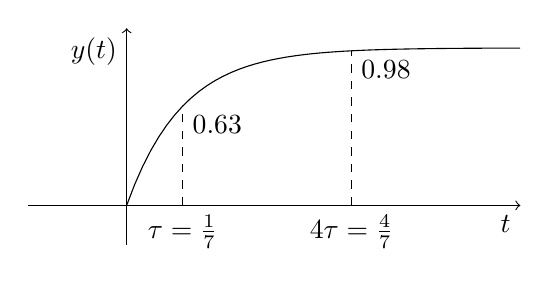
\begin{tikzpicture}[scale=2,xscale=2.5]
		\draw[->] (-0.25,0) -- (1,0) node[below left] {$ t $};  % x Axis
		\draw[->] (0,-0.25) -- (0,1.125) node[below left] {$ y(t) $};;  % y Axis
		
		\draw[domain=0:1,samples=50] plot (\x,{1-exp(-7*\x)});
		\draw[dashed] (1/7,0) node[below]{$ \tau=\frac{1}{7} $} -- ++(0,0.632) node[below right] {0.63};
		\draw[dashed] (4/7,0) node[below]{$ 4\tau=\frac{4}{7} $} -- ++(0,0.98) node[below right] {0.98};
	\end{tikzpicture}
\end{center}

%\exmp
%\[ Y(s)=\frac{s+1}{4s^2+15s+9} \]
%Find $ y(t) $. $ Y(s) $ is strictly proper. So, divide the numerator and denominator by 4.
%\[ Y(s)=\frac{\dfrac{s}{4}+\dfrac{1}{4}}{s^2+\dfrac{15}{4}s+\dfrac{9}{4}} = \frac{\dfrac{1}{4}(s+1)}{\left(s+\dfrac{3}{4}\right)(s+3)} \]
%Heaviside Expansion:
%\[ Y(s) = \frac{R_1}{s+\dfrac{3}{4}} + \frac{R_2}{s+3} \]
%where
%\[ R_1 = \left(s+\dfrac{3}{4}\right) \frac{\dfrac{1}{4}(s+1)}{\left(s+\dfrac{3}{4}\right)(s+3)}\Big|_{s=-3/4} = \frac{\dfrac{1}{4}(s+1)}{s+3}\Big|_{s=-3/4} = \frac{\dfrac{1}{4}(-\dfrac{3}{4}+1)}{-\dfrac{3}{4}+3} = \frac{\dfrac{1}{4}(\dfrac{1}{4})}{\dfrac{9}{4}} = \dfrac{1}{36} \]
%\[ R_2 = \left(s+3\right) \frac{\dfrac{1}{4}(s+1)}{\left(s+\dfrac{3}{4}\right)(s+3)}\Big|_{s=-3} = \frac{\dfrac{1}{4}(s+1)}{s+\dfrac{3}{4}}\Big|_{s=-3} = \frac{\dfrac{1}{4}(-3+1)}{-3+\dfrac{3}{4}} = \frac{\dfrac{1}{4}(-2)}{-\dfrac{9}{4}} = \dfrac{2}{9} \]
%So,
%\[ Y(s) = \frac{1/36}{s+3/4} + \frac{2/9}{s+3} \]
%Let's quickly check our work.
%\[ \frac{1/36}{s+3/4} + \frac{2/9}{s+3} = \frac{\dfrac{1}{36}(s+3)+\dfrac{2}{9}\left(s+\dfrac{3}{4}\right)}{\left(s+\dfrac{3}{4}\right)(s+3)} = \frac{s+3+8s+6}{36\left(s+\dfrac{15}{4}s+\dfrac{9}{4}\right)} = \frac{9s+9}{4\cdot9\cdot\left(s+\dfrac{15}{4}s+\dfrac{9}{4}\right)}  = \frac{s+1}{4s^2+15s+9} \quad\checkmark \]
%Then,
%\[ Y(s) = \frac{1/36}{s+3/4} + \frac{2/9}{s+3} \]
%\[ y(t) = \left(\frac{1}{36}e^{-\frac{3}{4}t} + \frac{2}{9}e^{-3t}\right)1(t) \]
%\[ y(t) = \frac{1}{36}\left(e^{-\frac{3}{4}t} + 8e^{-3t}\right)1(t) \]

%\exmp
%\[ \frac{dy}{dt} + 7y = 7\cdot1(t),\quad y(0^-)=0 \]
%Find $ y(t) $. First, take the Laplace transform.
%\[ sY(s)+7Y(s) = \frac{7}{s} \]
%Then solve for $ Y(s) $, expand, and find the residuals.
%\[ Y(s) = \frac{7}{s(s+7)} = \frac{R_1}{s}+\frac{R_2}{s+7} \]
%\[ R_1 = sY\Big|_{s=0}=1 \]
%\[ R_2 = (s+7)Y\Big|_{s=-7} = -1\]
%So,
%\[ Y(s) = \frac{1}{s}-\frac{1}{s+7} \]
%\[ y(t) = (1-e^{-7t})\cdot1(t) \]
%
%\begin{center}
%	\begin{tikzpicture}[scale=2]
%	\draw[->] (-0.5,0) -- (2,0);  % x Axis
%	\draw[->] (0,-0.25) -- (0,1.0);  % y Axis
%	\node[below left] at (2,0) {$ t $};
%	\node[below left] at (0,1) {$ y(t) $};
%	
%	\draw[domain=0:2,samples=50] plot (\x,{1-exp(-7*\x)});
%	\end{tikzpicture}
%\end{center}

\exmp
\[ \frac{d^2y}{dt^2} + 4y = 8\cdot1(t),\quad y(0^-)=0 \]
Find $ y(t) $. First, take the Laplace transform.
\[ s^2Y(s)+4Y(s) = \frac{8}{s} \]
Then solve for $ Y(s) $, expand, and find the residuals.
\[ Y(s) = \frac{8}{s(s^2+4)} = \frac{8}{s(s+2j)(s-2j)} =  \frac{R_1}{s}+\frac{R_2}{s+2j}+\frac{R_3}{s-2j} \]
\[ R_1 = sY\Big|_{s=0}=\frac{8}{4}=2 \]
\[ R_2 = (s+2j)Y\Big|_{s=-2j} = \frac{8}{-2j(-4j)} = -1\]
\[ R_3 = (s-2j)Y\Big|_{s=+2j} = \frac{8}{+2j(+4j)} = -1\]
So,
\[ Y(s) = \frac{2}{s}-\frac{1}{s+2j}-\frac{1}{s-2j} \]
\[ y(t)=\left(2-e^{2jt}-e^{-2jt}\right)1(t) = 2\left(1-\frac{e^{2jt}+e^{-2jt}}{2}\right) = 2\left(1-\cos(2t)\right)1(t) \]
$ \omega=2 $, so therefore the vibration period is $ T=\pi $.
\begin{center}
	\begin{tikzpicture}[scale=1]
	\draw[->] (-1,0) -- (8,0) node[below left] {$ t $};  % x Axis
	\draw[->] (0,-1) -- (0,5) node[below left] {$ y(t) $};  % y Axis
	
	\draw[domain=0:8,samples=500] plot (\x,{2-2*cos(\x*120)});
	\draw[dashed] (0,4) node[left] {4} -| (1.5,0) node[below] {$ \frac{\pi}{2} $};
	\draw (3,0) -- (3,-0.1) node[below] {$ \pi $};
	\draw[dashed] (4.5,4) -- (4.5,0) node[below] {$ \frac{3\pi}{2} $};
	\draw (6,0) -- (6,-0.1) node[below] {$ 2\pi $};
	\end{tikzpicture}
\end{center}

(returning to the procedure for inverse Laplace transform)
\begin{itemize}
	\item \textbf{Case B:} $ Y(s) $ is strictly proper but the $ p_k $'s are not distinct, i.e. there are some repeated roots. We'll demonstrate how to solve this with an example.
\end{itemize}
\exmp
\[ Y(s) = \frac{3}{(s+1)(s+2)^2} \]
Expanded:
\[ Y(s) = \frac{R_1}{s+1} + \frac{R_2}{(s+2)^2} + \frac{R_3}{s+2} \]
$ R_1 $ and $ R_2 $ are obtained the usual way.
\[ R_1 = (s+1)Y(s)\Big|_{s=-1} = 3 \]
\[ R_2 = (s+2)^2Y(s)\Big|_{s=-2} = -3 \]
$ R_3 $ is found as follows
\[ R_3 = \frac{d}{ds}\left[(s+2)^2Y(s)\right]\Big|_{s=-2} = \left(\frac{d}{ds}\frac{3}{s+1}\right)\Big|_{s=-2} = \frac{-3}{(s+1)^2}\Big|_{s=-2} = -3 \]
So,
\[ Y(s) = \frac{3}{s+1} - \frac{3}{(s+2)^2} - \frac{3}{s+2} = \overset{\text{check work:}}{\frac{3(s+2)^2-3(s+1)-3(s+1)(s+2)}{(s+1)(s+2)^2}} = \frac{3}{(s+1)(s+2)^2} \quad \checkmark \]
Then,
\[ y(t) = \left(3e^{-t} + \LT^{-1}\left[\frac{-3}{(s+2)^2}\right] -3e^{-2t}\right)1(t) \]
What is the inverse Laplace of $ \frac{-3}{(s+2)^2} $? Recall
\[ \LT[e^{-2t}\cdot1(t)] = \frac{1}{s+2} \]
\[ \LT[t\cdot e^{-2t}\cdot1(t)] = -\frac{d}{ds}\frac{1}{s+2}=\frac{1}{(s+2)^2} \]
So,
\[ y(t) = \left(3e^{-t} - 3te^{-2t}  -3e^{-2t} \right)1(t)\]

\exmp
\textbf{(Discussion Session)}
\[ Y(s) = \frac{2s+1}{s(s+1)^2} \]
Expanded:
\[ Y(s) = \frac{R_1}{s} + \frac{R_2}{(s+1)^2} + \frac{R_3}{s+1} \]
Find the residuals:
\[ R_1 = sY(s)\Big|_{s=0} = 1 \]
\[ R_2 = (s+1)^2Y(s)\Big|_{s=-1} = 1 \]
\[ R_3 = \frac{d}{ds}\left[(s+1)^2Y(s)\right]\Big|_{s=-1} = \frac{d}{ds}\frac{2s+1}{s}\Big|_{s=-1} = \frac{2s-(2s+1)}{s^2}\Big|_{s=-1} = \frac{-1}{s^2}\Big|_{s=-1} = -1 \]
So,
\[ Y(s) = \frac{1}{s} + \frac{1}{(s+1)^2} - \frac{1}{s+1} \]
Then,
\[ y(t) = \left(1 +te^{-t} -e^{-t}\right)1(t) \]

\exmp
\textbf{(Discussion Session)}
\[ Y(s) = \frac{3s+4}{s(s+1)^3} \]
Expanded:
\[ Y(s) = \frac{R_1}{s} + \frac{R_2}{(s+1)^3} + \frac{R_3}{(s+1)^2} + \frac{R_4}{s+1} \]
Find the residuals:
\[ R_1 = sY(s)\Big|_{s=0} = 4 \]
\[ R_2 = (s+1)^3Y(s)\Big|_{s=-1} = -1 \]
\[ R_3 = \frac{d}{ds}\left[(s+1)^3Y(s)\right]\Big|_{s=-1} = \frac{d}{ds}\frac{3s+4}{s}\Big|_{s=-1} = \frac{3s-(3s+4)}{s^2}\Big|_{s=-1} = \frac{-4}{s^2}\Big|_{s=-1} = -4 \]

\begin{align*}
R_4 &= \frac{1}{2!}\frac{d^2}{ds^2}\left[(s+1)^3Y(s)\right]\Big|_{s=-1} = \frac{1}{2}\frac{d^2}{ds^2}\frac{3s+4}{s}\Big|_{s=-1} \\
&=\frac{d}{ds}\frac{-4}{2s^2}\Big|_{s=-1} = \frac{4}{s^3}\Big|_{s=-1} = -4
\end{align*}
So,
\[ Y(s) = \frac{4}{s} - \frac{1}{(s+1)^3} - \frac{4}{(s+1)^2} - \frac{4}{s+1} \]
Then,
\[ y(t) = \left[4 -e^{-t}\left(\frac{1}{2}^2t+4t+4\right)\right]1(t) \]
How do we know
\[ \LT\left[\frac{1}{2}t^2e^{-t}1(t)\right]= \frac{1}{(s+1)^3} \ ? \]
We know
\[ \LT[te^{-t}]=\frac{1}{(s+1)^2} \]
So,
\[ \LT\left[t^2e^{-t}1(t)\right] = -\frac{d}{ds}\frac{1}{(s+1)^2} = \frac{2}{(s+1)^3} \]
\[ \LT\left[\frac{1}{2}t^2e^{-t}1(t)\right] = -\frac{d}{ds}\frac{1}{(s+1)^2} = \frac{1}{(s+1)^3} \]
\[ g(t) = \left(4 -\frac{1}{2}t^2e^{-t}-4te^{-t} -4e^{-t}\right)1(t) \]

We will now look at one final case:
\begin{itemize}
	\item \textbf{Case C:} $ Y(s) $ is proper and the $ p_k $'s are distinct. We'll demonstrate how to solve this with an example.
\end{itemize}

\exmp
\textbf{(Discussion Session)}
\[ Y(s)=\frac{s^2+1}{s^2+2s} = \frac{s^2+1}{s(s+2)} \]
This \textbf{won't work} if we try
\[ Y(s)= \frac{R_1}{s} + \frac{R_2}{s+2} \]
If we put this over a common denominator:
\[ Y(s)= \frac{(R_1+R_2)s+2R_1}{s(s+1)} \]
We can see that the degree of the numerator is too low! The solution is a modification to the Heaviside expansion:
\[ Y(s) = \frac{R_1}{s}+\frac{R_2}{s+2}+\mathbf{R_0} \]
Add something that will make the degree of the numerator ok. Adding a constant solves this problem. $ R_1 $ and $ R_2 $ are found the usual way.
\[ R_1 = sY(s)\Big|_{s=0} = \frac{1}{2} \]
\[ R_2 = (s+2)Y(s)\Big|_{s=-2} = -\frac{5}{2} \]
$ R_0 $ is found as follows:
\[ R_0 = \lim_{s\to\infty}Y(s) = 1 \]
So,
\[ Y(s) = \frac{1}{2s} - \frac{5}{2(s+2)} + 1 \]
\[ y(t) = \left(\frac{1}{2} - \frac{5}{2}e^{-2t}\right)1(t) + \delta(t) \]

This process is in fact the same with repeated poles, so we will not consider that a 4th case. We will show this with an example for repeated poles.
\exmp
\[ Y(s)=\frac{s^3+1}{s(s+2)^2} = \frac{s^3+1}{s^3+4s^2+4s} = \frac{R_1}{s} + \frac{R_2}{(s+2)^2} + \frac{R_3}{s+2} + R_0 \]
Then,
\[ R_1 = sY(s)\Big|_{s=0} = \frac{1}{4} \]
\[ R_2 = (s+2)^2Y(s)\Big|_{s=-2} = \frac{7}{2} \]
\[ R_3 = \frac{d}{ds}\left[(s+2)^2Y(s)\right]\Big|_{s=-2} =\frac{d}{ds}\frac{s^3+1}{s} = \frac{2s^3-1}{s^2} = -\frac{17}{4} \]

\[ R_0 = \lim_{s\to\infty}Y(s) = \lim_{s\to\infty} \frac{s^3+1}{s^3+4s^2+4s} = 1 \]
So,
\[ Y(s) = \frac{1}{4s} + \frac{7}{2(s+2)^2} - \frac{17}{4(s+2)} + 1 \]
\[ y(t) = \left(\frac{1}{4} - \frac{7}{2}te^{-2t} -\frac{17}{4}e^{-2t}  \right)1(t) + \delta(t) \]
\end{document}

